\documentclass[tikz,border=10pt]{standalone}
\usepackage{tikz}
\usepackage{pgfplots}
\pgfplotsset{compat=1.16}

\begin{document}

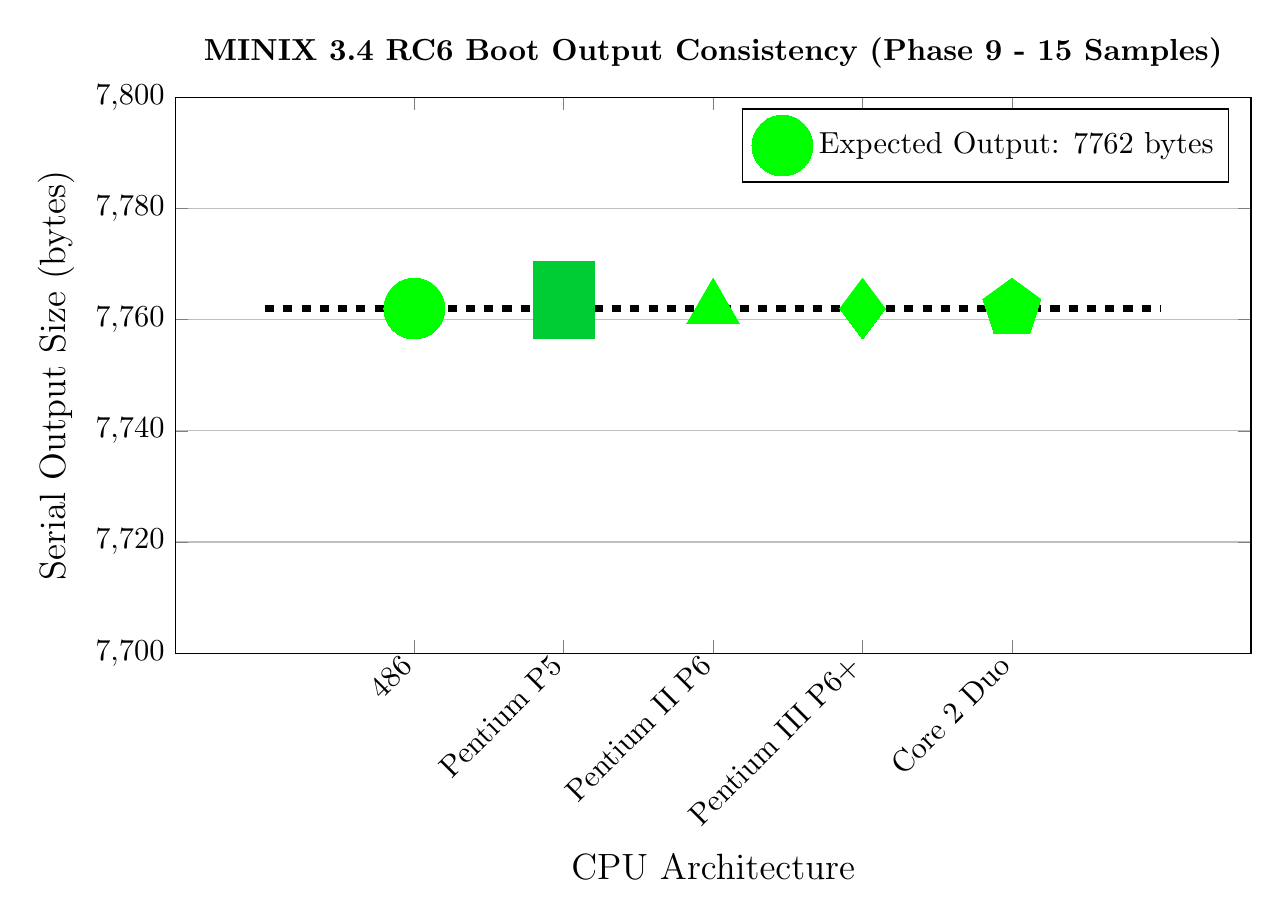
\begin{tikzpicture}[scale=1.1]
  \begin{axis}[
    title={MINIX 3.4 RC6 Boot Output Consistency (Phase 9 - 15 Samples)},
    xlabel={CPU Architecture},
    ylabel={Serial Output Size (bytes)},
    ymin=7700, ymax=7800,
    width=14cm,
    height=8cm,
    ymajorgrids=true,
    xtick={1,2,3,4,5},
    xticklabels={486, Pentium P5, Pentium II P6, Pentium III P6+, Core 2 Duo},
    x tick label style={rotate=45, anchor=east},
    ylabel style={font=\large},
    xlabel style={font=\large},
    title style={font=\Large, font=\bfseries},
    ]

    % Perfect consistency: 486 (3 samples at 7762 bytes)
    \addplot[color=green, mark=*, mark size=10pt, line width=0]
      coordinates {(1, 7762) (1, 7762) (1, 7762)};

    % Near-perfect: Pentium P5 (slight variance: 7765, 7762, 7762)
    \addplot[color=green!80!blue, mark=square*, mark size=10pt, line width=0]
      coordinates {(2, 7765) (2, 7762) (2, 7762)};

    % Perfect: Pentium II P6 (3 samples at 7762 bytes)
    \addplot[color=green, mark=triangle*, mark size=10pt, line width=0]
      coordinates {(3, 7762) (3, 7762) (3, 7762)};

    % Perfect: Pentium III P6+ (3 samples at 7762 bytes)
    \addplot[color=green, mark=diamond*, mark size=10pt, line width=0]
      coordinates {(4, 7762) (4, 7762) (4, 7762)};

    % Perfect: Core 2 Duo (3 samples at 7762 bytes)
    \addplot[color=green, mark=pentagon*, mark size=10pt, line width=0]
      coordinates {(5, 7762) (5, 7762) (5, 7762)};

    % Baseline reference line at 7762 bytes
    \addplot[color=black, line width=2pt, dashed, mark=none]
      coordinates {(0, 7762) (6, 7762)};
    \addlegendentry{Expected Output: 7762 bytes};

  \end{axis}
\end{tikzpicture}

\end{document}